\documentclass[dvipdfmx,11pt]{beamer}

%\usepackage{bxdpx-beamer}
\usepackage{listings,jlisting}
\usepackage{graphicx,xcolor} %文字の色
\usepackage[deluxe]{otf}
\usepackage{txfonts}


\usetheme{Warsaw}

\renewcommand{\kanjifamilydefault}{\gtdefault}
\renewcommand{\bibname}{参考文献}
\setbeamersize{text margin left=1.5em,text margin right=1.5em} %文字間の余白調整
\setbeamertemplate{navigation symbols}{} %アイコン消去
\setbeamertemplate{footline}[frame number] %フレーム番号表示
\useoutertheme{shadow}
\usefonttheme{professionalfonts} %数式文字のLaTeX化


\title{解集合プログラミングを用いたグラフ彩色問題の解法に関する考察}
\author{101830314 春田 穂高}
\institute{番原研究室}
\date{2021年度 卒業研究発表会\\2022年2月18日}

\begin{document}
%%%%%%%%%%%%%%%%%%%%%%%%%%%%%%%%%%%%%%%%%%%%%%%%%%%%%%%%%%%%%%%%%%%
\frame{\maketitle}
%%%%%%%%%%%%%%%%%%%%%%%%%%%%%%%%%%%%%%%%%%%%%%%%%%%%%%%%%%%%%%%%%%%

\begin{frame}{グラフ彩色問題と関連問題}

 \begin{itemize}
  \item \alert{グラフ彩色問題}
        \begin{itemize}
	 \item 与えられた有限無向グラフ $G$ の隣接する頂点が同色にならないように
	       各頂点を塗りわけるときに必要となる最小の色数を求める問題.
	 % \item 与えられた有限無向グラフ $G$ が彩色可能となるために
	 %       必要となる最小の色数を求める問題.
	 % \item グラフ $G$ の隣接する頂点が同色にならないように,$k$ 色で
	 %       各頂点を塗りわけられるとき,$k$ 彩色可能であるという.
         \item NP困難な問題である.
	 \item 最適化コンパイラのレジスタ割り付けや無線の周波数割り当てなどの応用がある.
        \end{itemize}
  \item \alert{グラフ彩色判定問題}
        \begin{itemize}
         \item 与えられた有限無向グラフ $G$ と色数 $k\ (\geq 3)$ に対して,
               $G$ が $k$ 色以下で彩色可能かどうかを判定する問題.
         \item NP完全な問題である.
        \end{itemize}
	 %%% 彩色数の説明(任意)
 \end{itemize}
 
\end{frame}

%%%%%%%%%%%%%%%%%%%%%%%%%%%%%%%%%%%%%%%%%%%%%%%%%%%%%%%%%%%%%%%%%%%

\begin{frame}{グラフ彩色問題と関連問題}
 \begin{itemize}
  \item \alert{グラフ彩色における同色頂点数最小化問題}
        \begin{itemize}
         \item グラフ彩色判定問題において,
               同色で彩色する頂点数の最小値を求める問題.
        \end{itemize}
  \item \alert{グラフ彩色における同色頂点数最大化問題}
        \begin{itemize}
         \item グラフ彩色判定問題において,
               同色で彩色する頂点数の最大値を求める問題.
        \end{itemize}
  \item \alert{グラフ彩色における多色頂点数最大化問題}
        \begin{itemize}
         \item グラフ彩色問題において,
               2色以上で彩色できる頂点数の最大値を求める問題.
         \item この問題の最適解は,基のグラフ彩色判定問題の複数の実行可能解に
               対応する圧縮解とみなすことができる.
	 %%% 解の圧縮の話を入れる
        \end{itemize}

 \end{itemize}
 
\end{frame}

%%%%%%%%%%%%%%%%%%%%%%%%%%%%%%%%%%%%%%%%%%%%%%%%%%%%%%%%%%%%%%%%%%%
\begin{frame}{McGregorグラフ[Knuth2015]\cite{Knuth:TAOCP:SAT}}
 \begin{exampleblock}{order~$5$のMcGregorグラフ}
  \begin{center}
   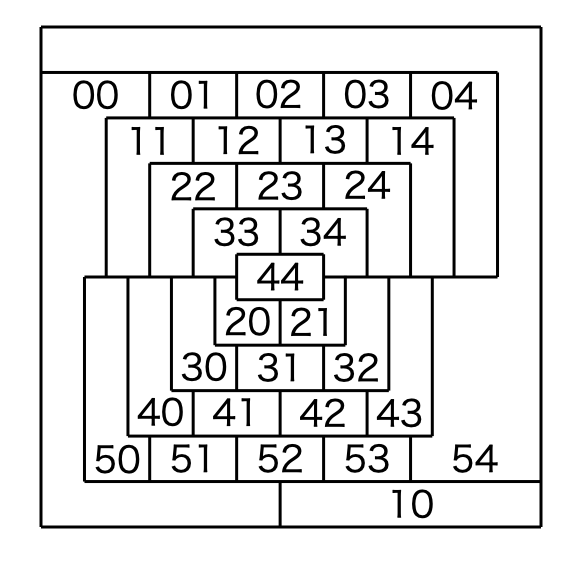
\includegraphics[scale=0.2]{fig/order5.png}
  \end{center}
  % \begin{itemize}
  %  \item 頂点数: 30
  %  \item 辺数: 84
  % \end{itemize}
 \end{exampleblock}

 \begin{itemize}
  % \item D.~E~.Knuthの教科書
  %        The Art of Computer Programming~\cite{Knuth:TAOCP:SAT}
  %        に記載されているグラフである.
  \item グラフを構成する頂点や辺は,order~$n$ によって定まる.
  \item 頂点数:\,$N=n*(n+1)$個\quad 辺数:\,$3N-6$本.

  \item McGregorグラフは,いずれも4彩色可能なグラフである.
 \end{itemize}
 
\end{frame}

%%%%%%%%%%%%%%%%%%%%%%%%%%%%%%%%%%%%%%%%%%%%%%%%%%%%%%%%%%%%%%%%%%%

\begin{frame}{多色頂点数最大化問題の例}
\begin{tabular}{cc}
 \begin{minipage}[t]{0.5\linewidth}
  \centering
  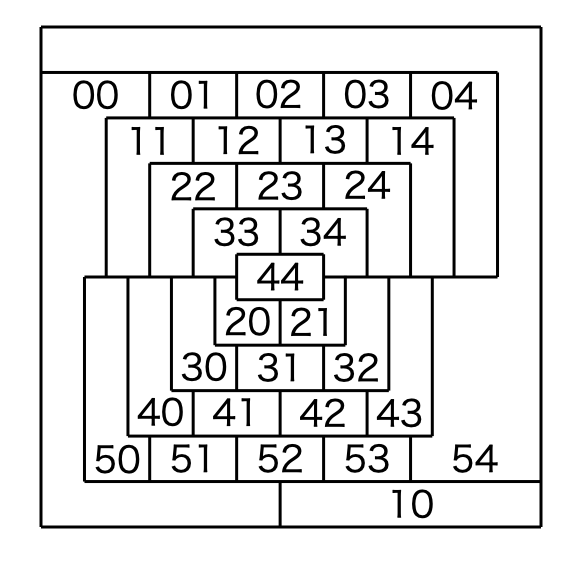
\includegraphics[scale=0.2]{fig/order5.png}
 \end{minipage}
 \begin{minipage}[t]{0.5\linewidth}
  \centering
  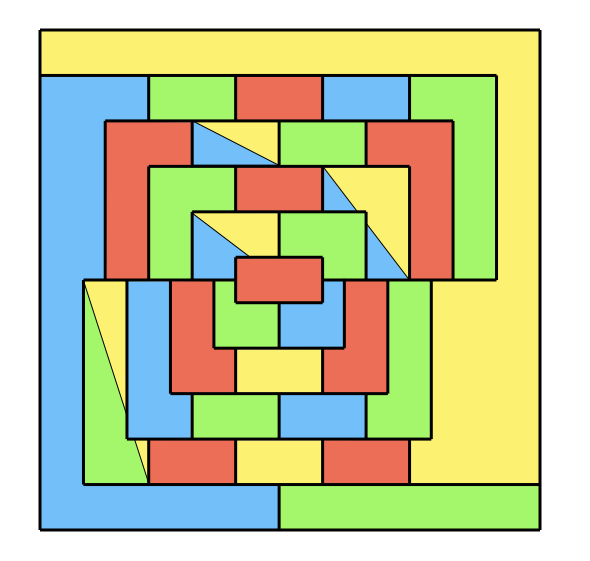
\includegraphics[scale=0.2]{fig/order5_mult.png}
 \end{minipage}
\end{tabular}

\begin{exampleblock}{}
 order $5$ の McGregorグラフが与えられた時に,
 2色以上の色で彩色できる頂点数の最大値を求める問題を考える.%%% 問題文の追加
\end{exampleblock}

\begin{alertblock}{}
 \begin{itemize}
  \item 12,24,33,50の4頂点が多色で彩色できる.
  \item この最適解は基のグラフ彩色判定問題の実行可能解の
        $2^4=$\alert{\textbf{16}}通りを
        圧縮した解とみなすことができる.%%% もっと詳細に
 \end{itemize}
\end{alertblock}

\end{frame}

%%%%%%%%%%%%%%%%%%%%%%%%%%%%%%%%%%%%%%%%%%%%%%%%%%%%%%%%%%%%%%%%%%%

\begin{frame}{解集合プログラミング(Answer Set Programming; ASP)}

 \begin{itemize}
  \item \alert{ASP}は,論理プログラミングから派生した
        比較的新しいプログラミングパラダイムである.
  \item \alert{ASP言語}は,一階論理に基づいた知識表現言語の一種である.
  \item \alert{ASPシステム}は,論理プログラムから
        安定モデル意味論~{\scriptsize[Gelfond and Lifschitz, '88]}
        に基づく解集合を計算するシステムである.
  \item 近年,SAT技術を利用する高速なASPシステムが開発され,
        様々な分野への実用的な応用が急速に拡大している.
 \end{itemize}
 
 \begin{alertblock}{グラフ彩色判定問題に対してASPを用いる利点}
  \begin{itemize}
   \item ASP言語の高い表現力により,制約を簡潔に記述可能.
   \item 充足不能コアを用いた最適化探索が可能.
   \item 高速ASPシステムを用いた高速な解探索,解列挙が可能.
  \end{itemize}
 \end{alertblock}
 
\end{frame}

%%%%%%%%%%%%%%%%%%%%%%%%%%%%%%%%%%%%%%%%%%%%%%%%%%%%%%%%%%%%%%%%%%%

\begin{frame}{研究目的と内容}

 \begin{alertblock}{研究目的}%%% 未定
  \begin{itemize}
   \item グラフ彩色判定問題とその関連問題に対して,
         ASP符号化を提案し,評価する.
   \item 得られた解を利用した,グラフ彩色問題の実行可能解の圧縮.
  \end{itemize}

 \end{alertblock}

 \begin{block}{研究内容}
  \begin{enumerate}
   \item \structure{グラフ彩色判定問題とその関連問題を解くASP符号化の考案}
         \begin{itemize}
          \item %color符号化,
                minimize符号化,
                maximize符号化,mult符号化.
         \end{itemize}
   \item \structure{ベンチマーク問題を用いた評価実験}
         \begin{itemize}
%          \item McGregorグラフを表すベンチマーク問題(計138問)を新たに作成.
          \item グラフ彩色判定問題,同色頂点数最小化問題,
                同色頂点数最大化問題,多色頂点数最大化問題
                のそれぞれに対する実験を行った.
          \item グラフ彩色判定問題の実行可能解の全解列挙.%%% 未定
         \end{itemize}
   \item \structure{グラフ彩色判定問題の実行可能解の圧縮についての調査}
         \begin{itemize}
          \item 多色頂点数最大化問題の一つの解が基のグラフ彩色判定問題の
                実行可能解の何通りを圧縮している解なのかを調査を行った.
         \end{itemize}
  \end{enumerate}
 \end{block}
 
\end{frame}

%%%%%%%%%%%%%%%%%%%%%%%%%%%%%%%%%%%%%%%%%%%%%%%%%%%%%%%%%%%%%%%%%%%

\begin{frame}{ 考案するASP符号化}
%%% 大幅な変更
 \begin{block}{グラフ彩色判定問題の表現}
  与えられた有限無向グラフ $G$ で以下の2つの制約を満たす時,
  必要となる最小の色数を求める問題.
  \begin{itemize}
   \item $G$の各頂点は一つの色で彩色される.(彩色制約)
   \item $G$の隣接する頂点は同色で彩色されない.(隣接制約)
  \end{itemize}
 \end{block}
 \begin{enumerate}
   \item \alert{color符号化}:
         \begin{itemize}
          \item グラフ彩色判定問題の彩色制約と隣接制約を,
                ASPの個数制約,一貫制約を用いて簡潔に記述.
         \end{itemize}
  \item \alert{minimize符号化}:
        \begin{itemize}
         \item color符号化に,%同色頂点数最小化問題の目的関数を
               ASPの最小化関数を追加.%%% もっと詳細の説明でもいいかも
        \end{itemize}
  \item \alert{maximize符号化}:
        \begin{itemize}
         \item color符号化に,%同色頂点数最大化問題の目的関数を
               ASPの最大化関数を追加.
        \end{itemize}
  \item \alert{mult符号化}:
        \begin{itemize}
         \item color符号化をベースに,
               頂点を彩色する色の数をASPの個数制約の上限を緩和し,
               多色で彩色できるように定義.
               %%% color符号化はベースとしていいの?
               %%% minimizeとmaximizeの「ベースに」と同義?
               %%% 変更よりも定義
         \item ASPの最大化関数を用いて多色で彩色できる頂点数を最大化するよう記述.
        \end{itemize}
 \end{enumerate}
\end{frame}

%%%%%%%%%%%%%%%%%%%%%%%%%%%%%%%%%%%%%%%%%%%%%%%%%%%%%%%%%%%%%%%%%%%

% \begin{frame}{実験概要}
%  \begin{block}{}
%   考案した符号化の有効性を評価するために各問題の実験を行った.
%  \end{block}

% \begin{itemize}
%  \item \structure{ベンチマーク問題}: order~3$\sim$140のMcGregorグラフ(計138問)
%  \item \structure{ASPシステム}: \textit{clingo}-5.5.0
%  \item \structure{実験環境}: Mac mini Intel Core i7 3.2GHz 64GBメモリ
%  \item \structure{制限時間}: 
%        \begin{itemize}%%% 問題に対してでなくて良いか
%         \item color符号化: 30分
%         \item minimize,maximize,mult符号化: 1時間
%        \end{itemize}
% \end{itemize}  

%  \begin{alertblock}{color符号化の実験結果}
%   order~3$\sim$138の計136問について4彩色可能であると判定できた.
%  \end{alertblock}
 
% \end{frame}

%%%%%%%%%%%%%%%%%%%%%%%%%%%%%%%%%%%%%%%%%%%%%%%%%%%%%%%%%%%%%%%%%%%

\begin{frame}{実験概要}
 \begin{block}{}
  考案した符号化の有効性を評価するために各問題の実験を行った.
 \end{block}

\begin{itemize}
 \item \structure{対象とする問題}:
       \begin{enumerate}
        \item グラフ彩色判定問題: McGregorグラフ~order~3$\sim$140の計138問
              \begin{itemize}
               \item \structure{制限時間}: 30分/問
              \end{itemize}
        \item 同色頂点数最小化問題: McGregorグラフ~order~3$\sim$20の計18問
              \begin{itemize}
               \item \structure{制限時間}: 1時間/問
              \end{itemize}
        \item 同色頂点数最大化問題: McGregorグラフ~order~3$\sim$38の計36問
              \begin{itemize}
               \item \structure{制限時間}: 1時間/問
              \end{itemize}
        \item 多色頂点数最大化問題: McGregorグラフ~order~3$\sim$15の計13問
              \begin{itemize}
               \item \structure{制限時間}: 1時間/問
              \end{itemize}
       \end{enumerate}
 \item \structure{ASPシステム}: \textit{clingo}-5.5.0
 \item \structure{実験環境}: Mac mini Intel Core i7 3.2GHz 64GBメモリ
\end{itemize}  

 \begin{alertblock}{color符号化の実験結果}
  order~3$\sim$138の計136問について4彩色可能であると判定できた.
 \end{alertblock}
 
\end{frame}

%%%%%%%%%%%%%%%%%%%%%%%%%%%%%%%%%%%%%%%%%%%%%%%%%%%%%%%%%%%%%%%%%%%

\begin{frame}{実験結果:同色頂点数最小化問題}

 \begin{block}{}
  \structure{問題}: order\ n~$=$~3$\sim$20のMcGregorグラフ(計18問)
 \end{block}

 \begin{center}
  \begin{tabular}{r|c|c}
 %n& f(n)\\
 N&BB &USC\\
 \hline
 3&2*&2*\\
 4&2*&2*\\
 5&3*&3*\\
 6&4*&4*\\
 7&5*&5*\\
 8&7*&7*\\
 9&7*&7*\\
 10&7*&7*\\
 11&8*&8*\\
 12&9*&9*\\
 13&10*&10*\\
 14&12&\textbf{12*}\\
 15&\textbf{12}&49\\
 16&16&\textbf{12*}\\
 17&21&\textbf{\textcolor{red}{13*}}\\
 18&19&\textbf{\textcolor{red}{14*}}\\
 19&\textbf{20}&58\\
 20&\textbf{22}&59\\\hline
\end{tabular}


 \end{center}

 \begin{itemize}
  \item BB法が優れていた問題は3問,
        USC法が優れていた問題は4問.
  \item BB法では11問,USC法では15問,最適値を求めることができた.
  \item order~17,18の2問について新たに最適値を発見することができた.
 \end{itemize}
 
\end{frame}

%%%%%%%%%%%%%%%%%%%%%%%%%%%%%%%%%%%%%%%%%%%%%%%%%%%%%%%%%%%%%%%%%%%

\begin{frame}{実験結果:同色頂点数最大化問題}

 \begin{block}{}
  \structure{問題数}: order\ n~$=$~3$\sim$38のMcGregorグラフ(計36問)
  %%% 最小化と同じ形式で
 \end{block}
 
 \begin{center}
  \begin{table}[t]\scriptsize
%\renewcommand{\arraystrech}{1.2}
\begin{tabular}{r|cc||r|cc||r|cc}
 \hline
 %n& g(n)\\
 N&BB &USC&N&BB&USC&N&BB&USC\\
 \hline
 3&4*&4*&    15&71&\textbf{77*}&
 27&\textbf{185}&180 \\
 4&6*&6*&    16&71&\textbf{88*}&
 28&199&\textbf{\textcolor{red}{266*}} \\
 5&10*&10*&    17&76&\textbf{\textcolor{red}{99*}}&
 29&221&\textbf{\textcolor{red}{285*}} \\
 6&13*&13*&    18&91&\textbf{\textcolor{red}{111*}}&
 30&224&\textbf{\textcolor{red}{305*}} \\
 7&17*&17*&    19&92&\textbf{\textcolor{red}{123*}}&
 31&247&\textbf{\textcolor{red}{325*}} \\
 8&23*&23*&    20&109&\textbf{\textcolor{red}{137*}}&
 32&255&255 \\
 9&28&\textbf{28*}&    21&121&\textbf{\textcolor{red}{150*}}&
 33&\textbf{280}&278 \\
 10&35&\textbf{35*}&    22&122&\textbf{\textcolor{red}{165*}}&
 34&296&\textbf{\textcolor{red}{391*}} \\
 11&42&\textbf{42*}&    23&137&\textbf{\textcolor{red}{180*}}&
 35&310&\textbf{\textcolor{red}{414*}} \\
 12&49&\textbf{50*}&    24&146&\textbf{\textcolor{red}{196*}}&
 36&338&\textbf{\textcolor{red}{438*}} \\
 13&56&\textbf{58*}&    25&162&\textbf{\textcolor{red}{212*}}&
 37&\textbf{348}&340 \\
 14&56&\textbf{68*}&    26&180&\textbf{\textcolor{red}{230*}}&
 38&371&371 \\ 
\end{tabular}
\end{table}

 \end{center}

 \begin{itemize}
  \item BB法が優れていた問題は3問,
        USC法が優れていた問題は25問.
  \item BB法では6問,USC法が31問,最適値を求めることができた.
  \item 17問について新たに最適値を発見することができた.
 \end{itemize}

\end{frame}

%%%%%%%%%%%%%%%%%%%%%%%%%%%%%%%%%%%%%%%%%%%%%%%%%%%%%%%%%%%%%%%%%%%

\begin{frame}{実験結果:多色頂点数最大化問題}

 \begin{block}{}
  \structure{問題数}: order\ n~$=$~3$\sim$15のMcGregorグラフ(計13問)
  %%% 最小化と同じ形式で
 \end{block}
 
 \begin{center}
  \begin{tabular}{r|r|r}
 %n& h(n)\\
 N&BB &USC\\
 \hline
 3&1*&1*\\
 4&3*&3*\\
 5&4*&4*\\
 6&7*&7*\\
 7&9*&9*\\
 8&13*&13*\\
 9&18*&18*\\
 10&23&\textbf{23*}\\
 11&27&\textbf{\textcolor{red}{29*}}\\
 12&34&\textbf{\textcolor{red}{36*}}\\
 13&\textbf{39}&15\\
 14&\textbf{44}&11\\
 15&\textbf{49}&20\\\hline
\end{tabular}


 \end{center}

 \begin{itemize}
  \item BB法が優れていた問題は3問,
        USC法が優れていた問題は3問.%%% (BB法が優れていた問題は何問....)
  \item BB法では7問,USC法では10問,最適値を求めることができた.
  \item order~11,12の2問について新たに
        最適値を発見することができた.%%% 17, 18...
 \end{itemize}

\end{frame}

%%%%%%%%%%%%%%%%%%%%%%%%%%%%%%%%%%%%%%%%%%%%%%%%%%%%%%%%%%%%%%%%%%%

\begin{frame}{実行可能解の圧縮}
%%% h(n)の説明
 \begin{block}{}
  多色頂点数最大化問題の一つの解が基のグラフ彩色判定問題の
  実行可能解の何通りを圧縮している解なのかを調査を行った.
 \end{block}
 
 \begin{center}
  \begin{tabular}{r|c|c|c}
 \hline
 n& h(n)& 圧縮された解の個数& 圧縮率 \\
 \hline
 3&	1&	2&	1.3889 \\
 4&	3&	8&	0.3367 \\
 5&	4&	16&	0.0368 \\
 6&	7&	128&	0.0049 \\
 7&	9&	512&	0.0002 \\
 8&	13&	8192&	- \\
 9&	18&	262144&	- \\
 10&	23&	8388608&	- \\
 11&	29&	536870912&	- \\
 12&	36&	68719476736&	- \\
\end{tabular}
\caption{多色頂点数最大化問題の解の圧縮率}
\label{table:com}
 \end{center}

 \begin{itemize}
  \item 多色頂点数最大化問題で最適値を発見できた
        order3$\sim$12までの計10問の解の圧縮に成功した.
  \item order12では約680億もの実行可能解を表していることがわかった.
 \end{itemize}

\end{frame}

%%%%%%%%%%%%%%%%%%%%%%%%%%%%%%%%%%%%%%%%%%%%%%%%%%%%%%%%%%%%%%%%%%%

\begin{frame}{まとめと今後の課題}

 \begin{enumerate}
  \item \structure{グラフ彩色判定問題とその関連問題を解くASP符号化の提案}
        \begin{itemize}
         \item ASPの高い表現力により簡潔に記述できることが確認できた.
        \end{itemize}
  \item \structure{ベンチマーク問題を用いた評価実験}
        \begin{itemize}
         \item グラフ彩色判定問題,同色頂点数最小化問題,
               同色頂点数最大化問題,多色頂点数最大化問題
               のそれぞれに対する実験を行った.
         \item 同色頂点数最小化問題,同色頂点数最大化問題.多色頂点数最大化問題
               のそれぞれに対して,新たに最適値を発見した.
         \item グラフ彩色判定問題の実行可能解の全解列挙に成功した.%%% 未定
        \end{itemize}
  \item \structure{グラフ彩色判定問題の実行可能解の圧縮についての調査}
        \begin{itemize}
         \item 多色頂点数最大化問題で発見した10問の最適値について
               基のグラフ彩色判定問題の実行可能解の圧縮することに成功した.
        \end{itemize}
 \end{enumerate}

 \begin{block}{今後の課題}
  \begin{itemize}
   \item ASP符号化の改良
         \begin{itemize}
          \item 対称性の除去の実装等.
         \end{itemize}
   \item McGregorグラフ以外のグラフでの評価実験
  \end{itemize}
 \end{block}
 
\end{frame}

%%%%%%%%%%%%%%%%%%%%%%%%%%%%%%%%%%%%%%%%%%%%%%%%%%%%%%%%%%%%%%%%%%%

\begin{frame}[noframenumbering]{参考文献}
 \bibliographystyle{jplain} % 参考文献スタイル
 \bibliography{aisat,bachelor}    % 参考文献リスト
\end{frame}

%%%%%%%%%%%%%%%%%%%%%%%%%%%%%%%%%%%%%%%%%%%%%%%%%%%%%%%%%%%%%%%%%%%

\begin{frame}[noframenumbering]{}
 \thispagestyle{empty}
 \Huge 付録
\end{frame}

%%%%%%%%%%%%%%%%%%%%%%%%%%%%%%%%%%%%%%%%%%%%%%%%%%%%%%%%%%%%%%%%%%%

\begin{frame}[noframenumbering]{グラフ彩色問題の実行可能解の全解列挙(1/2)}
 \thispagestyle{empty}

 \begin{block}{}
  %グラフ彩色における多色頂点数最大化問題の実行可能解の圧縮を確認するために,
  グラフ彩色問題の実行可能解の全解列挙する実験を行った.  
 \end{block}

 \begin{block}{実験概要}
  \begin{itemize}
   \item \structure{ASPシステム}: \textit{clingo}-5.5.0
   \item \structure{実験環境}: Mac mini Intel Core i7 3.2GHz 64GBメモリ
   \item \structure{制限時間}: 1時間
   \item \structure{問題数}: McGregorグラフのorder3$\sim$10までの計8問
  \end{itemize}
 \end{block}
\end{frame}

%%%%%%%%%%%%%%%%%%%%%%%%%%%%%%%%%%%%%%%%%%%%%%%%%%%%%%%%%%%%%%%%%%%

\begin{frame}[noframenumbering]{グラフ彩色問題の実行可能解の全解列挙(2/2)}
 \thispagestyle{empty}

 \begin{center}
  \begin{tabular}{r|r|r}
 \hline
 N& 解の総数& CPU時間\\
 3&144*&0.002\\
 4&2376*&0.009\\
 5&43536*&0.143\\
 6&2589768*&7.796\\
 7&224442336*&865.500\\
 8&$\geq$816623222&-\\
 9&$\geq$676088853&-\\
 10&$\geq$504392039&-\\
\end{tabular}

 \end{center}

 \begin{itemize}
  \item order3$\sim$7までの計5問について全解列挙に成功した.
 \end{itemize}
\end{frame}

%%%%%%%%%%%%%%%%%%%%%%%%%%%%%%%%%%%%%%%%%%%%%%%%%%%%%%%%%%%%%%%%%%%
\end{document}

%%% Local Variables:
%%% mode: japanese-latex
%%% TeX-master: 
%%% End: